\begin{minipage}[c]{\textwidth}
\advance\leftskip-2.5cm
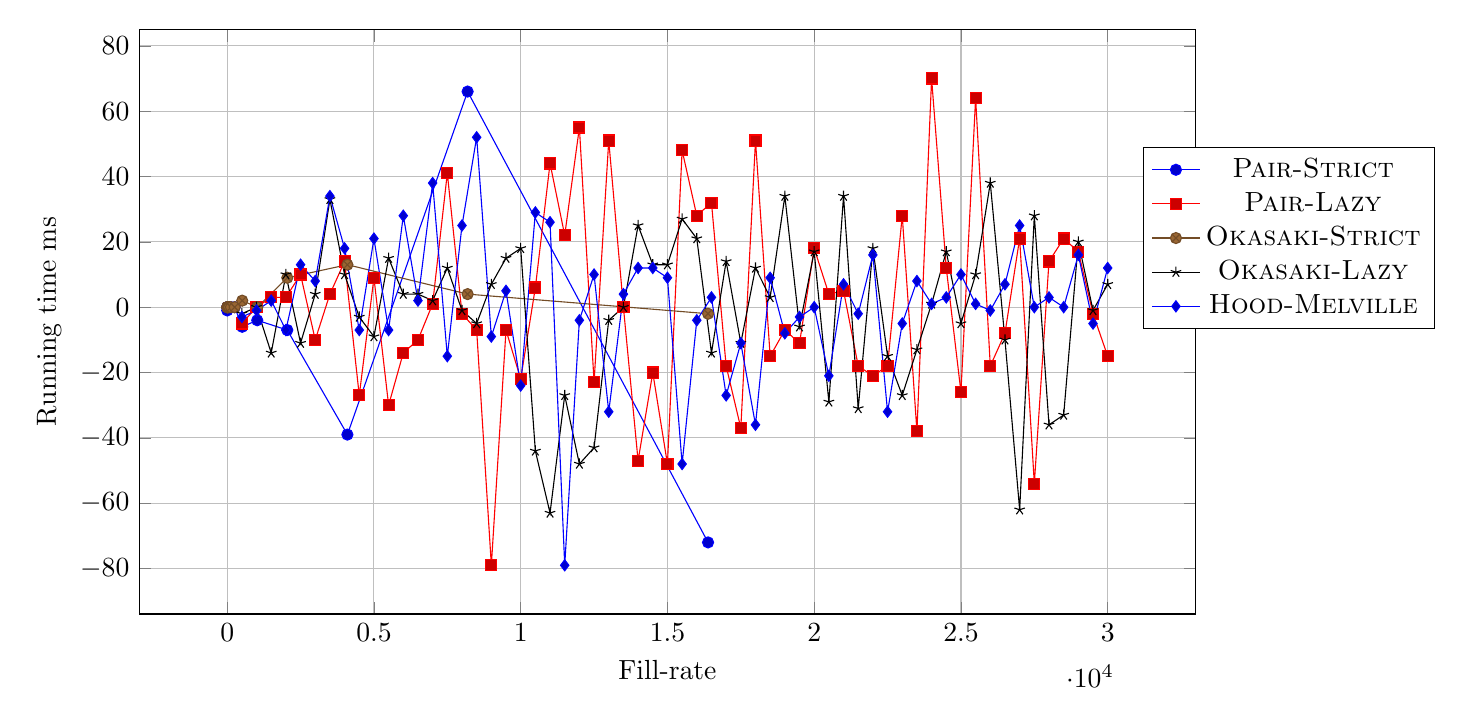
\begin{tikzpicture}
        \begin{axis}[
            xlabel = Fill-rate,
            ylabel = Running time ms,
            height=9cm,
            width=15cm,
            grid=major,
            legend style={
            at={(0.95,0.8)},
            anchor=north west}]            
            legend pos=center west
    	]
    		
  
                \addplot coordinates {
(1,-1)
(2,0)
(4,0)
(8,0)
(16,0)
(32,0)
(64,0)
(128,0)
(256,0)
(512,-6)
(1024,-4)
(2048,-7)
(4096,-39)
(8192,66)
(16384,-72)

    	};
        
    	\addlegendentry{\textsc{Pair-Strict}}

        \addplot coordinates {
(500,-5)
(1000,0)
(1500,3)
(2000,3)
(2500,10)
(3000,-10)
(3500,4)
(4000,14)
(4500,-27)
(5000,9)
(5500,-30)
(6000,-14)
(6500,-10)
(7000,1)
(7500,41)
(8000,-2)
(8500,-7)
(9000,-79)
(9500,-7)
(10000,-22)
(10500,6)
(11000,44)
(11500,22)
(12000,55)
(12500,-23)
(13000,51)
(13500,0)
(14000,-47)
(14500,-20)
(15000,-48)
(15500,48)
(16000,28)
(16500,32)
(17000,-18)
(17500,-37)
(18000,51)
(18500,-15)
(19000,-7)
(19500,-11)
(20000,18)
(20500,4)
(21000,5)
(21500,-18)
(22000,-21)
(22500,-18)
(23000,28)
(23500,-38)
(24000,70)
(24500,12)
(25000,-26)
(25500,64)
(26000,-18)
(26500,-8)
(27000,21)
(27500,-54)
(28000,14)
(28500,21)
(29000,17)
(29500,-2)
(30000,-15)

    	};
        
    	\addlegendentry{\textsc{Pair-Lazy}}

        \addplot coordinates {
(1,0)
(2,0)
(4,0)
(8,0)
(16,0)
(32,0)
(64,0)
(128,0)
(256,0)
(512,2)
(1024,0)
(2048,9)
(4096,13)
(8192,4)
(16384,-2)

    	};
        
    	\addlegendentry{\textsc{Okasaki-Strict}}

        \addplot coordinates {
(500,-2)
(1000,0)
(1500,-14)
(2000,10)
(2500,-11)
(3000,4)
(3500,33)
(4000,10)
(4500,-3)
(5000,-9)
(5500,15)
(6000,4)
(6500,4)
(7000,2)
(7500,12)
(8000,-1)
(8500,-5)
(9000,7)
(9500,15)
(10000,18)
(10500,-44)
(11000,-63)
(11500,-27)
(12000,-48)
(12500,-43)
(13000,-4)
(13500,0)
(14000,25)
(14500,13)
(15000,13)
(15500,27)
(16000,21)
(16500,-14)
(17000,14)
(17500,-11)
(18000,12)
(18500,3)
(19000,34)
(19500,-6)
(20000,17)
(20500,-29)
(21000,34)
(21500,-31)
(22000,18)
(22500,-15)
(23000,-27)
(23500,-13)
(24000,1)
(24500,17)
(25000,-5)
(25500,10)
(26000,38)
(26500,-10)
(27000,-62)
(27500,28)
(28000,-36)
(28500,-33)
(29000,20)
(29500,-1)
(30000,7)

    	};
        
    	\addlegendentry{\textsc{Okasaki-Lazy}}

        \addplot coordinates {
(500,-3)
(1000,-1)
(1500,2)
(2000,-7)
(2500,13)
(3000,8)
(3500,34)
(4000,18)
(4500,-7)
(5000,21)
(5500,-7)
(6000,28)
(6500,2)
(7000,38)
(7500,-15)
(8000,25)
(8500,52)
(9000,-9)
(9500,5)
(10000,-24)
(10500,29)
(11000,26)
(11500,-79)
(12000,-4)
(12500,10)
(13000,-32)
(13500,4)
(14000,12)
(14500,12)
(15000,9)
(15500,-48)
(16000,-4)
(16500,3)
(17000,-27)
(17500,-11)
(18000,-36)
(18500,9)
(19000,-8)
(19500,-3)
(20000,0)
(20500,-21)
(21000,7)
(21500,-2)
(22000,16)
(22500,-32)
(23000,-5)
(23500,8)
(24000,1)
(24500,3)
(25000,10)
(25500,1)
(26000,-1)
(26500,7)
(27000,25)
(27500,0)
(28000,3)
(28500,0)
(29000,16)
(29500,-5)
(30000,12)

    	};

    	\addlegendentry{\textsc{Hood-Melville}}

        \end{axis}

    \end{tikzpicture}
    \captionof{figure}{TITEL}
    \label{fig:sample_figure}
\end{minipage}